% !Mode:: "TeX:UTF-8"
% !TEX program = xelatex

\def\usewhat{xelatex}                               
\documentclass[12pt,openany,oneside]{ctexbook}
                                                     % 本科生毕业论文通常采用单页排版
%!Tex Program = xelatex
% -*-coding: utf-8 -*-


\usepackage{graphicx}

%\usepackage[a4paper,text={162true mm,249true mm},left=24true mm,
%            head=24true mm, top=24true mm, bottom=24true mm,
%           headheight=14true mm, headsep=10true mm
%           ]{geometry}% 东北林业大学要求的宽度

%\usepackage[a4paper,]{geometry}%四周都是24mm
\usepackage[a4paper,
left=24true mm,right=24true mm, top=25true mm, bottom=23true mm,
headheight=14true mm,
headsep=7true mm,
footskip=7true mm]{geometry}% 东北林业大学要求的宽度
\usepackage{layout}


\usepackage{titlesec}               % 控制标题的宏包
\usepackage{titletoc}                   % 控制目录的宏包
\usepackage{fancyhdr}                   % fancyhdr宏包 页眉和页脚的相关定义
%\usepackage[UTF8]{ctex}
\usepackage{color}          % 支持彩色
\usepackage{amsmath}        % AMSLaTeX宏包 用来排出更加漂亮的公式
\usepackage{amssymb}
\usepackage{epsfig}         % eps图像
\usepackage[below]{placeins}%允许上一个section 的浮动图形出现在下一个section的开始部分,还提供\FloatBarrier命令,使所有未处理的浮动图形立即被处理
\usepackage{flafter}       % 使得所有浮动体不能被放置在其浮动环境之前,以免浮动体在引述它的文本之前出现.
\usepackage{multirow}       %使用Multirow宏包,使得表格可以合并多个row 格
\usepackage{booktabs}       % 表格,横的粗线;\specialrule{1pt}{0pt}{0pt}
\usepackage{longtable}      %支持跨页的表格。
\usepackage{tabularx}
\usepackage{subfigure}%支持子图 %centerlast 设置最后一行是否居中
\usepackage[subfigure]{ccaption} %支持双语标题
\usepackage[sort&compress,numbers]{natbib}% 支持引用缩写的宏包
\makeatletter
%林大的参考文献研究用波浪链接~
\def\NAT@citexnum[#1][#2]#3{%
  \NAT@reset@parser
  \NAT@sort@cites{#3}%
  \NAT@reset@citea
  \@cite{\def\NAT@num{-1}\let\NAT@last@yr\relax\let\NAT@nm\@empty
    \@for\@citeb:=\NAT@cite@list\do
    {\@safe@activestrue
     \edef\@citeb{\expandafter\@firstofone\@citeb\@empty}%
     \@safe@activesfalse
     \@ifundefined{b@\@citeb\@extra@b@citeb}{%
       {\reset@font\bfseries?}
        \NAT@citeundefined\PackageWarning{natbib}%
       {Citation `\@citeb' on page \thepage \space undefined}}%
     {\let\NAT@last@num\NAT@num\let\NAT@last@nm\NAT@nm
      \NAT@parse{\@citeb}%
      \ifNAT@longnames\@ifundefined{bv@\@citeb\@extra@b@citeb}{%
        \let\NAT@name=\NAT@all@names
        \global\@namedef{bv@\@citeb\@extra@b@citeb}{}}{}%
      \fi
      \ifNAT@full\let\NAT@nm\NAT@all@names\else
        \let\NAT@nm\NAT@name\fi
      \ifNAT@swa
       \@ifnum{\NAT@ctype>\@ne}{%
        \@citea
        \NAT@hyper@{\@ifnum{\NAT@ctype=\tw@}{\NAT@test{\NAT@ctype}}{\NAT@alias}}%
       }{%
        \@ifnum{\NAT@cmprs>\z@}{%
         \NAT@ifcat@num\NAT@num
          {\let\NAT@nm=\NAT@num}%
          {\def\NAT@nm{-2}}%
         \NAT@ifcat@num\NAT@last@num
          {\@tempcnta=\NAT@last@num\relax}%
          {\@tempcnta\m@ne}%
         \@ifnum{\NAT@nm=\@tempcnta}{%
          \@ifnum{\NAT@merge>\@ne}{}{\NAT@last@yr@mbox}%
         }{%
           \advance\@tempcnta by\@ne
           \@ifnum{\NAT@nm=\@tempcnta}{%
             \ifx\NAT@last@yr\relax
               \def@NAT@last@yr{\@citea}%
             \else
               \def@NAT@last@yr{$\sim$\NAT@penalty}%
             \fi
           }{%
             \NAT@last@yr@mbox
           }%
         }%
        }{%
         \@tempswatrue
         \@ifnum{\NAT@merge>\@ne}{\@ifnum{\NAT@last@num=\NAT@num\relax}{\@tempswafalse}{}}{}%
         \if@tempswa\NAT@citea@mbox\fi
        }%
       }%
       \NAT@def@citea
      \else
        \ifcase\NAT@ctype
          \ifx\NAT@last@nm\NAT@nm \NAT@yrsep\NAT@penalty\NAT@space\else
            \@citea \NAT@test{\@ne}\NAT@spacechar\NAT@mbox{\NAT@super@kern\NAT@@open}%
          \fi
          \if*#1*\else#1\NAT@spacechar\fi
          \NAT@mbox{\NAT@hyper@{{\citenumfont{\NAT@num}}}}%
          \NAT@def@citea@box
        \or
          \NAT@hyper@citea@space{\NAT@test{\NAT@ctype}}%
        \or
          \NAT@hyper@citea@space{\NAT@test{\NAT@ctype}}%
        \or
          \NAT@hyper@citea@space\NAT@alias
        \fi
      \fi
     }%
    }%
      \@ifnum{\NAT@cmprs>\z@}{\NAT@last@yr}{}%
      \ifNAT@swa\else
        \@ifnum{\NAT@ctype=\z@}{%
          \if*#2*\else\NAT@cmt#2\fi
        }{}%
        \NAT@mbox{\NAT@@close}%
      \fi
  }{#1}{#2}%
}%
\makeatother

\usepackage{enumitem}       %使用enumitem宏包,改变列表项的格式
\usepackage{calc}           %长度可以用+ - * / 进行计算


%%\usepackage{txfonts}
\usepackage{mathtools}

\usepackage{bm}              % 处理数学公式中的黑斜体的宏包

% 生成有书签的pdf及其开关, 该宏包应放在所有宏包的最后, 宏包之间有冲突
\def\atemp{dvipdfmx}\ifx\atemp\usewhat
\usepackage[dvipdfm,unicode,           %dvi-->pdf 生成书签
            bookmarksnumbered=true,
            bookmarksopen=true,
            colorlinks=false,
            pdfborder={0 0 1},
            citecolor=blue,
            linkcolor=red,
            anchorcolor=green,
            urlcolor=blue,
            breaklinks=true
            ]{hyperref}
\fi

\def\atemp{pdflatex}\ifx\atemp\usewhat
\usepackage{cmap}                       %pdflatex编译时,可以生成可复制、粘贴的中文PDF 文档
\usepackage[pdftex,unicode,
            %CJKbookmarks=true,
            bookmarksnumbered=true,
            bookmarksopen=true,
            colorlinks=false,
            pdfborder={0 0 1},
            citecolor=blue,
            linkcolor=red,
            anchorcolor=green,
            urlcolor=blue,
            breaklinks=true
            ]{hyperref}
\fi

\def\atempxetex{xelatex}\ifx\atempxetex\usewhat %\def\atempxetex{xelatex} main.tex中已定义;



\usepackage[xetex,
            bookmarksnumbered=true,
            bookmarksopen=true,
            colorlinks=false,
            pdfborder={0 0 1},
            citecolor=blue,
            linkcolor=red,
            anchorcolor=green,
            urlcolor=blue,
            breaklinks=true,
            naturalnames  %与algorithm2e宏包协调
            ]{hyperref}
%\usepackage{fontenc}
%xunicode xunicode Ross Moore’s xunicode package is now automatically loaded for users of both XELATEX and LuaLATEX.
\usepackage[BoldFont,SlantFont]{xeCJK}
\defaultfontfeatures{Mapping=tex-text}

\xeCJKsetemboldenfactor{1}%只对随后定义的CJK字体有效
\setCJKfamilyfont{hei}{SimHei}
\xeCJKsetemboldenfactor{4}
\setCJKfamilyfont{song}{SimSun}
\xeCJKsetemboldenfactor{1}
\setCJKfamilyfont{fs}{FangSong}
\setCJKfamilyfont{kai}{KaiTi}
\setCJKfamilyfont{li}{LiSu}
\setCJKfamilyfont{xw}{STXinwei}

\setCJKmainfont{SimSun}
\setmainfont{Times New Roman}
\setsansfont{Arial}

\newcommand{\hei}{\CJKfamily{hei}}% 黑体   (Windows自带simhei.ttf)
\newcommand{\song}{\CJKfamily{song}}    % 宋体   (Windows自带simsun.ttf)
\newcommand{\fs}{\CJKfamily{fs}}        % 仿宋体 (Windows自带simfs.ttf)
\newcommand{\kai}{\CJKfamily{kai}}      % 楷体   (Windows自带simkai.ttf)
\newcommand{\li}{\CJKfamily{li}}        % 隶书   (Windows自带simli.ttf)
\newcommand{\xw}{\CJKfamily{xw}}        % 隶书   (Windows自带simli.ttf)


\newfontfamily\arial{Arial}
\newfontfamily\timesnewroman{Times New Roman}

%
\fi

\usepackage[boxed,linesnumbered,algochapter]{algorithm2e}%\let\chapter\undefined
% 算法的宏包,注意宏包兼容性,先后顺序为float、hyperref、algorithm(2e),否则无法生成算法列表

\usepackage{setspace}%更改行距的宏包
%\usepackage{syntonly}检查语法不编译
%\syntaxonly
\usepackage{tikz}%R语言作图使用
\usepackage{xltxtra}%输出XeLaTeX
							% 定义本文所使用宏包
\graphicspath{figures/}							% 定义所有的图像文件在 figures 子目录下

\begin{document}								% 开始全文
% !Mode:: "TeX:UTF-8"
%  Authors: 张井   Jing Zhang: prayever@gmail.com     天津大学2010级管理与经济学部信息管理与信息系统专业硕士生
%           余蓝涛 Lantao Yu: lantaoyu1991@gmail.com  天津大学2008级精密仪器与光电子工程学院测控技术与仪器专业本科生

%%%%%%%%%%%%%%%%% Fonts Definition and Basics %%%%%%%%%%%%%%%%%
\setCJKfamilyfont{思源黑体}{Noto Sans CJK SC}
\setCJKfamilyfont{思源宋体}{Noto Serif CJK SC}
\newcommand{\hei}{\CJKfamily{思源黑体}}
\newcommand{\song}{\CJKfamily{思源宋体}}
\newcommand{\yihao}{\fontsize{26pt}{26pt}\selectfont}       % 一号, 单倍行距
\newcommand{\xiaoyi}{\fontsize{24pt}{24pt}\selectfont}      % 小一, 单倍行距
\newcommand{\erhao}{\fontsize{22pt}{1.25\baselineskip}\selectfont}       % 二号, 1.25倍行距
\newcommand{\xiaoer}{\fontsize{18pt}{18pt}\selectfont}      % 小二, 单倍行距
\newcommand{\sanhao}{\fontsize{16pt}{16pt}\selectfont}      % 三号, 单倍行距
\newcommand{\xiaosan}{\fontsize{15pt}{15pt}\selectfont}     % 小三, 单倍行距
\newcommand{\sihao}{\fontsize{14pt}{14pt}\selectfont}       % 四号, 单倍行距
\newcommand{\xiaosi}{\fontsize{12pt}{12pt}\selectfont}      % 小四, 单倍行距
\newcommand{\wuhao}{\fontsize{10.5pt}{10.5pt}\selectfont}   % 五号, 单倍行距
\newcommand{\xiaowu}{\fontsize{9pt}{9pt}\selectfont}        % 小五, 单倍行距

%\CJKtilde  % 重新定义了波浪符~的意义
% JUST DON'T USE CJK
% 使用 ctexbook 之后已无必要
\newcommand\prechaptername{第}
\newcommand\postchaptername{章}

\punctstyle{hangmobanjiao}             % 调整中文字符的表示,行内占一个字符宽度,行尾占半个字符宽度

% 调整罗列环境的布局
\setitemize{leftmargin=3em,itemsep=0em,partopsep=0em,parsep=0em,topsep=-0em}
\setenumerate{leftmargin=3em,itemsep=0em,partopsep=0em,parsep=0em,topsep=0em}

% 避免宏包 hyperref 和 arydshln 不兼容带来的目录链接失效的问题。
\def\temp{\relax}
\let\temp\addcontentsline
\gdef\addcontentsline{\phantomsection\temp}

% 自定义项目列表标签及格式 \begin{publist} 列表项 \end{publist}
\newcounter{pubctr} %自定义新计数器
\newenvironment{publist}{%%%%%定义新环境
\begin{list}{[\arabic{pubctr}]} %%标签格式
    {
     \usecounter{pubctr}
     \setlength{\leftmargin}{2.5em}   % 左边界 \leftmargin =\itemindent + \labelwidth + \labelsep
     \setlength{\itemindent}{0em}     % 标号缩进量
     \setlength{\labelsep}{1em}       % 标号和列表项之间的距离,默认0.5em
     \setlength{\rightmargin}{0em}    % 右边界
     \setlength{\topsep}{0ex}         % 列表到上下文的垂直距离
     \setlength{\parsep}{0ex}         % 段落间距
     \setlength{\itemsep}{0ex}        % 标签间距
     \setlength{\listparindent}{0pt}  % 段落缩进量
    }}
{\end{list}}

\makeatletter
\renewcommand\normalsize{
  \@setfontsize\normalsize{12pt}{12pt} % 小四对应 12 pt
  \setlength\abovedisplayskip{4pt}
  \setlength\abovedisplayshortskip{4pt}
  \setlength\belowdisplayskip{\abovedisplayskip}
  \setlength\belowdisplayshortskip{\abovedisplayshortskip}
  \let\@listi\@listI}
\def\defaultfont{\renewcommand{\baselinestretch}{1.63}\normalsize\selectfont} % 设置行距

\renewcommand{\CJKglue}{\hskip -0.1 pt plus 0.08\baselineskip} % 控制字间距,使每行 34 个汉字
\makeatother

%%%%%%%%%%%%% Contents %%%%%%%%%%%%%%%%%
\renewcommand{\contentsname}{目\qquad 录}
\setcounter{tocdepth}{2} % 控制目录深度
% 使用 ctexbook 之后已无必要
%\titlecontents{chapter}[2em]{\vspace{.5\baselineskip}\xiaosan\song}
             %{\prechaptername\CJKnumber{\thecontentslabel}\postchaptername\qquad}{}
             %{\hspace{.5em}\titlerule*[10pt]{$\cdot$}\sihao\contentspage}
\titlecontents{chapter}[2em]{\vspace{.5\baselineskip}\xiaosan\song}
             {\thecontentslabel\!\!\qquad}{}
             {\titlerule*[5pt]{$\cdot$}\sihao\contentspage}
\titlecontents{section}[3em]{\vspace{.25\baselineskip}\sihao\song}
             {\thecontentslabel\quad}{}
             {\titlerule*[5pt]{$\cdot$}\sihao\contentspage}
\titlecontents{subsection}[4em]{\vspace{.25\baselineskip}\sihao\song}
             {\thecontentslabel\quad}{}
             {\titlerule*[5pt]{$\cdot$}\sihao\contentspage}

%%%%%%%%%% Chapter and Section %%%%%%%%%%%%%
\setcounter{secnumdepth}{4}
\setlength{\parindent}{2em}
\renewcommand{\chaptername}{\prechaptername\CJKnumber{\thechapter}\postchaptername}
\titleformat{\chapter}{\centering\xiaosan\hei}{\chaptername}{2em}{}
\titlespacing{\chapter}{0pt}{0.1\baselineskip}{0.8\baselineskip}
\titleformat{\section}{\sihao\hei}{\thesection}{1em}{}
\titlespacing{\section}{0pt}{0.15\baselineskip}{0.25\baselineskip}
\titleformat{\subsection}{\sihao\hei}{\thesubsection}{1em}{}
\titlespacing{\subsection}{0pt}{0.1\baselineskip}{0.3\baselineskip}
\titleformat{\subsubsection}{\sihao\hei}{\thesubsubsection}{1em}{}
\titlespacing{\subsubsection}{0pt}{0.05\baselineskip}{0.1\baselineskip}

\newcommand{\trtitle}[1]{\vspace{12pt}\begin{center}{\xiaoer\hei\bf #1}\end{center}}
\newcommand{\trchapter}[1]{\vspace{6pt}{\raggedright\xiaosan\hei #1}\newline}
\newcommand{\trsection}[1]{\vspace{4pt}{\raggedright\sihao\hei #1}\newline}
\newcommand{\trsubsection}[1]{\vspace{2pt}{\raggedright\sihao\hei\it #1}\newline}

%%%%%%%%%% Table, Figure and Equation %%%%%%%%%%%%%%%%%
\renewcommand{\tablename}{表}                                     % 插表题头
\renewcommand{\figurename}{图}                                    % 插图题头
\renewcommand{\thefigure}{\arabic{chapter}-\arabic{figure}}       % 使图编号为 7-1 的格式 %\protect{~}
\renewcommand{\thesubfigure}{\alph{subfigure})}                   % 使子图编号为 a) 的格式
\renewcommand{\thesubtable}{(\alph{subtable})}                    % 使子表编号为 (a) 的格式
\renewcommand{\thetable}{\arabic{chapter}-\arabic{table}}         % 使表编号为 7-1 的格式
\renewcommand{\theequation}{\arabic{chapter}-\arabic{equation}}   % 使公式编号为 7-1 的格式
\newcommand{\ud}{\mathrm{d}}

%%%%%% 定制浮动图形和表格标题样式 %%%%%%
\makeatletter
\long\def\@makecaption#1#2{
   \vskip\abovecaptionskip
   \sbox\@tempboxa{\centering\wuhao\song{#1\qquad #2} }
   \ifdim \wd\@tempboxa >\hsize
     \centering\wuhao\song{#1\qquad #2} \par
   \else
     \global \@minipagefalse
     \hb@xt@\hsize{\hfil\box\@tempboxa\hfil}
   \fi
   \vskip\belowcaptionskip\vspace{8pt}}
\makeatother
\captiondelim{~~~~} %用来控制longtable表头分隔符

%%%%%%%%%% Theorem Environment %%%%%%%%%%%%%%%%%
\theoremstyle{plain}
\theorembodyfont{\song\rmfamily}
\theoremheaderfont{\hei\rmfamily}
\newtheorem{theorem}{定理~}[chapter]
\newtheorem{lemma}{引理~}[chapter]
\newtheorem{axiom}{公理~}[chapter]
\newtheorem{proposition}{命题~}[chapter]
\newtheorem{prop}{性质~}[chapter]
\newtheorem{corollary}{推论~}[chapter]
\newtheorem{definition}{定义~}[chapter]
\newtheorem{conjecture}{猜想~}[chapter]
\newtheorem{example}{例~}[chapter]
\newtheorem{remark}{注~}[chapter]
%\newtheorem{algorithm}{算法~}[chapter]
\newenvironment{proof}{\noindent{\hei 证明:}}{\hfill $ \square $ \vskip 4mm}
\theoremsymbol{$\square$}

%%%%%%%%%% Page: number, header and footer  %%%%%%%%%%%%%%%%%

%\frontmatter 或 \pagenumbering{roman}
%\mainmatter 或 \pagenumbering{arabic}
\makeatletter
\renewcommand\frontmatter{\clearpage
  \@mainmatterfalse
  }
\makeatother

%%%%%%%%%%% Code: Listings from MCM Template %%%%%%%%%%%%

\definecolor{grey}{rgb}{0.8,0.8,0.8}
\definecolor{darkgreen}{rgb}{0,0.3,0}
\definecolor{darkblue}{rgb}{0,0,0.3}
\def\lstbasicfont{\fontfamily{pcr}\selectfont\footnotesize}
\lstset{%
% indexing
   % numbers=left,
   % numberstyle=\small,%
% character display
    showstringspaces=false,
    showspaces=false,%
    tabsize=4,%
% style
    frame=lines,%
    basicstyle={\footnotesize\lstbasicfont},%
    keywordstyle=\color{darkblue}\bfseries,%
    identifierstyle=,%
    commentstyle=\color{darkgreen},%\itshape,%
    stringstyle=\color{black}%
}
\lstloadlanguages{C,C++,Java,Matlab,Mathematica,Python}

%%%%%%%%%%%% References %%%%%%%%%%%%%%%%%

\makeatletter
\renewenvironment{thebibliography}[1]{
   \wuhao
   \list{\@biblabel{\@arabic\c@enumiv}}
        {\renewcommand{\makelabel}[1]{##1\hfill}
         \settowidth\labelwidth{0 cm}
         \setlength{\labelsep}{0pt}
         \setlength{\itemindent}{0pt}
         \setlength{\leftmargin}{\labelwidth+\labelsep}
         \addtolength{\itemsep}{-0.7em}
         \usecounter{enumiv}
         \let\p@enumiv\@empty
         \renewcommand\theenumiv{\@arabic\c@enumiv}}
    \sloppy\frenchspacing
    \clubpenalty4000
    \@clubpenalty \clubpenalty
    \widowpenalty4000
    \interlinepenalty4000
    \sfcode`\.\@m}
   {\def\@noitemerr
     {\@latex@warning{Empty 'thebibliography' environment}}
    \endlist\frenchspacing}
\makeatother

\addtolength{\bibsep}{-0.5em}     % 缩小参考文献间的垂直间距
\setlength{\bibhang}{2em}         % 每个条目自第二行起缩进的距离

% 参考文献引用作为上标出现
\newcommand{\citeup}[1]{\textsuperscript{\cite{#1}}}

%%%%%%%%%%%% Cover %%%%%%%%%%%%%%%%%
% 封面、摘要、版权、致谢格式定义
\makeatletter
\def\ctitle#1{\def\@ctitle{#1}}\def\@ctitle{}
\def\cdegree#1{\def\@cdegree{#1}}\def\@cdegree{}
\def\caffil#1{\def\@caffil{#1}}\def\@caffil{}
\def\csubject#1{\def\@csubject{#1}}\def\@csubject{}
\def\cgrade#1{\def\@cgrade{#1}}\def\@cgrade{}
\def\cauthor#1{\def\@cauthor{#1}}\def\@cauthor{}
\def\cnumber#1{\def\@cnumber{#1}}\def\@cnumber{}
\def\csupervisor#1{\def\@csupervisor{#1}}\def\@csupervisor{}
\def\crank#1{\def\@crank{#1}}\def\@crank{}
\def\cdate#1{\def\@cdate{#1}}\def\@cdate{}
\long\def\cabstract#1{\long\def\@cabstract{#1}}\long\def\@cabstract{}
\long\def\eabstract#1{\long\def\@eabstract{#1}}\long\def\@eabstract{}
\def\ckeywords#1{\def\@ckeywords{#1}}\def\@ckeywords{}
\def\ekeywords#1{\def\@ekeywords{#1}}\def\@ekeywords{}
\def\cheading#1{\def\@cheading{#1}}\def\@cheading{}


\pagestyle{fancy}
\fancyhf{}
\fancyhead[C]{\song\wuhao \@cheading}  % 页眉显示天津大学 20XX 届本科生毕业论文
\fancyfoot[C]{\song\xiaowu ~\thepage~}
\newlength{\@title@width}

%%%%%%%%%%%%%%%%%%%     Cover     %%%%%%%%%%%%%%%%%%%%%%%
\def\makecover{
   	\phantomsection
    \pdfbookmark[-1]{\@ctitle}{ctitle}

    \begin{titlepage}
      	\vspace*{31.5pt}
      	\begin{center}
  			\begin{figure}[h]
  				\centering
  				
\includegraphics[width=0.4\textwidth]{figures/tjuname}
  			\end{figure}
  			\vspace*{21pt}
  			\hei\erhao{\textbf{本科生毕业论文}}
  			\vspace*{52.5pt}

  			\begin{figure}[h]
  				\centering
  				
\includegraphics[width=0.4\textwidth]{figures/tjulogo}
  			\end{figure}
  			\vspace*{42pt}
  			
  			\renewcommand\arraystretch{1.5}
  			\setlength{\@title@width}{5cm}{\song\sanhao{\textbf{
    			\begin{tabular}{lc}
      				学\qquad 院&	\underline{\makebox[\@title@width][c]{\@caffil}}	\\
      				专\qquad 业&	\underline{\makebox[\@title@width][c]{\@csubject}}	\\
      				年\qquad 级&	\underline{\makebox[\@title@width][c]{\@cgrade}}	\\
      				姓\qquad 名&	\underline{\makebox[\@title@width][c]{\@cauthor}} 	\\
      				指导教师   &	\underline{\makebox[\@title@width][c]{\@csupervisor}} \\
  				\end{tabular}
  			}}}
  			\vspace*{21pt}

			\song\sanhao{\textbf{\@cdate}}
		\end{center}
	\end{titlepage}
}

%%%%%%%%%%%%%%%%%%%    Abstract    %%%%%%%%%%%%%%%%%%%%%%%
\def\makeabstract{
	\titleformat{\chapter}{\centering\sanhao\hei}{\chaptername}{2em}{} %"摘要"三号黑体居中

%%%%% Chinese Abstract %%%%%
	\clearpage
	\markboth{摘~要}{摘~要}
	\pdfbookmark[0]{摘~~要}{cabstract}
	\chapter*{摘\qquad 要}
	
	\song\defaultfont
	\@cabstract
	\vspace{\baselineskip}

	\hangafter=1\hangindent=52.3pt\noindent
	{\hei\xiaosi 关键词:} \@ckeywords
	\thispagestyle{empty}

%%%%% English Abstract %%%%%
	\clearpage
	\markboth{ABSTRACT}{ABSTRACT}
	\pdfbookmark[0]{ABSTRACT}{eabstract}
	\chapter*{\bf{ABSTRACT}}
	
	\@eabstract
	\vspace{\baselineskip}

	\hangafter=1\hangindent=60pt\noindent
	{\textbf{Keywords:}} \@ekeywords
	\thispagestyle{empty}
}

%%%%%%%%%%%%%%%%%%%    Contents    %%%%%%%%%%%%%%%%%%%%%%%
\def\makecontents{
	\titleformat{\chapter}{\centering\sanhao\hei}{\chaptername}{2em}{} %"目录"三号黑体居中

	\clearpage{\pagestyle{empty}\cleardoublepage}
	\pdfbookmark[0]{目~~录}{mulu}
	\tableofcontents                                     % 中文目录
	\fancypagestyle{plain}{
		\fancyhf{}
		\renewcommand{\headrulewidth}{0 pt}
		\fancyfoot[C]{\song\xiaowu~\thepage~}
	}
	\thispagestyle{plain}

	\mainmatter\defaultfont\sloppy\raggedbottom
	\makeatletter
	\fancypagestyle{plain}{                              % 设置开章页眉页脚风格
    	\fancyhf{}
    	\fancyhead[C]{\song\wuhao \@cheading}            % 首页页眉格式
    	\fancyfoot[C]{\song\xiaowu ~\thepage~}           % 首页页脚格式
    	\renewcommand{\headrulewidth}{0.5pt}
    	\renewcommand{\footrulewidth}{0pt}
	}
}

%%%%%%%%%%%%%%%%%%%   References   %%%%%%%%%%%%%%%%%%%%%%%
\def\makereferences{
	\titleformat{\chapter}{\raggedright\sihao\hei}{\chaptername}{2em}{} % "参考文献"四号黑体顶格
	\chapter*{\bibname}
	\defaultfont
	\bibliographystyle{references/ref.bst}
	\bibliography{references/ref}

	\phantomsection
	\markboth{参考文献}{参考文献}
	\addcontentsline{toc}{chapter}{参考文献}       % 参考文献加入到中文目录
	\nocite{*}                                     % 若将此命令屏蔽掉,则未引用的文献不会出现在文后的参考文献中
}

\makeatother

							% 完成对论文各个部分格式的设置
\frontmatter									% 以下是论文导言部分,包括论文的封面,中英文摘要和中文目录
\fancypagestyle{plain}{
	\fancyhf{}
	\renewcommand{\headrulewidth}{0 pt}
	\fancyfoot[C]{\song\xiaowu~\thepage~}
}

%%%%%%%%%%    封面    %%%%%%%%%%
\tongjisetup{
  %******************************
  % 注意:
  %   1. 配置里面不要出现空行
  %   2. 不需要的配置信息可以删除
  %******************************
  %
  %=====
  % 秘级
  %=====
  secretlevel={保密},
  secretyear={2},
  %
  %=========
  % 中文信息
  %=========
  % 题目过长可以换行(推荐手动加入换行符,这样就可以控制换行的地方啦)。
  ctitle={同济大学学位论文 \LaTeX{} 模板\\使用示例说明与参考},
  cheadingtitle={同济大学学位论文 \LaTeX{} 模板使用示例说明与参考},    %用于页眉的标题,不要换行
  cauthor={同济人},  
  studentnumber={201804},
  cmajorfirst={工学},
  cmajorsecond={电子控制计算机},
  cdepartment={同济大学Linux用户组},
  csupervisor={陈杰 教授}, 
  % 如果没有副指导老师或者校外指导老师,把{}中内容留空即可,或者直接注释掉。
  cassosupervisor={裴刚 教授~(校外)}, % 副指导老师
  % 日期自动使用当前时间,若需手动指定,按如下方式修改:
  % cdate={\zhdigits{2018}年\zhnumber{11}月},
  % 没有基金的话就注释掉吧。
  cfunds={(本论文由我要努力想办法撑到两行的著名国家杰出青年基金 (No.123456789) 支持)},
  %
  %=========
  % 英文信息
  %=========
  etitle={A Simple Sample of Tongji Thesis\\ Using \tongjithesis{}}, 
  eauthor={Tongji Ren},
  emajorfirst={Gong Xue},
  emajorsecond={DianziControlComputerScience},
  edepartment={TONGJILUG},
  % 日期自动使用当前时间,若需手动指定,按如下方式修改:
  % edate={November,\ 2018},
  efunds={(Supported by the Natural Science Foundation of China for\\ Distinguished Young Scholars, Grant No.123456789)},    
  esupervisor={Prof. Jie Chen},
  eassosupervisor={Prof. Gang Pei (XiaoWai)}
  }

% 定义中英文摘要和关键字
\begin{cabstract}  
  论文的摘要是对论文研究内容和成果的高度概括。摘要应对论文所研究的问题及其研究目
  的进行描述,对研究方法和过程进行简单介绍,对研究成果和所得结论进行概括。摘要应
  具有独立性和自明性,其内容应包含与论文全文同等量的主要信息。使读者即使不阅读全
  文,通过摘要就能了解论文的总体内容和主要成果。

  论文摘要的书写应力求精确、简明。切忌写成对论文书写内容进行提要的形式,尤其要避
  免“第 1 章……;第 2 章……;……”这种或类似的陈述方式。

  本文介绍同济大学论文模板 \tongjithesis{} 的使用方法。本模板符合学校的硕士、
  博士论文格式要求。

  本文的创新点主要有:
  \begin{itemize}
    \item 用例子来解释模板的使用方法;
    \item 用废话来填充无关紧要的部分;
    \item 一边学习摸索一边编写新代码。
  \end{itemize}

  关键词是为了文献标引工作、用以表示全文主要内容信息的单词或术语。关键词不超过 5
  个,每个关键词中间用分号分隔。(模板作者注:关键词分隔符不用考虑,模板会自动处
  理。英文关键词同理。)
\end{cabstract}

\ckeywords{\TeX, \LaTeX, CJK, 模板, 论文}

\begin{eabstract}
   An abstract of a dissertation is a summary and extraction of research work
   and contributions. Included in an abstract should be description of research
   topic and research objective, brief introduction to methodology and research
   process, and summarization of conclusion and contributions of the
   research. An abstract should be characterized by independence and clarity and
   carry identical information with the dissertation. It should be such that the
   general idea and major contributions of the dissertation are conveyed without
   reading the dissertation.

   An abstract should be concise and to the point. It is a misunderstanding to
   make an abstract an outline of the dissertation and words ``the first
   chapter'', ``the second chapter'' and the like should be avoided in the
   abstract.

   Key words are terms used in a dissertation for indexing, reflecting core
   information of the dissertation. An abstract may contain a maximum of 5 key
   words, with semi-colons used in between to separate one another.
\end{eabstract}

\ekeywords{\TeX, \LaTeX, CJK, template, thesis}

%%%%%%%%%%   任务书   %%%%%%%%%%
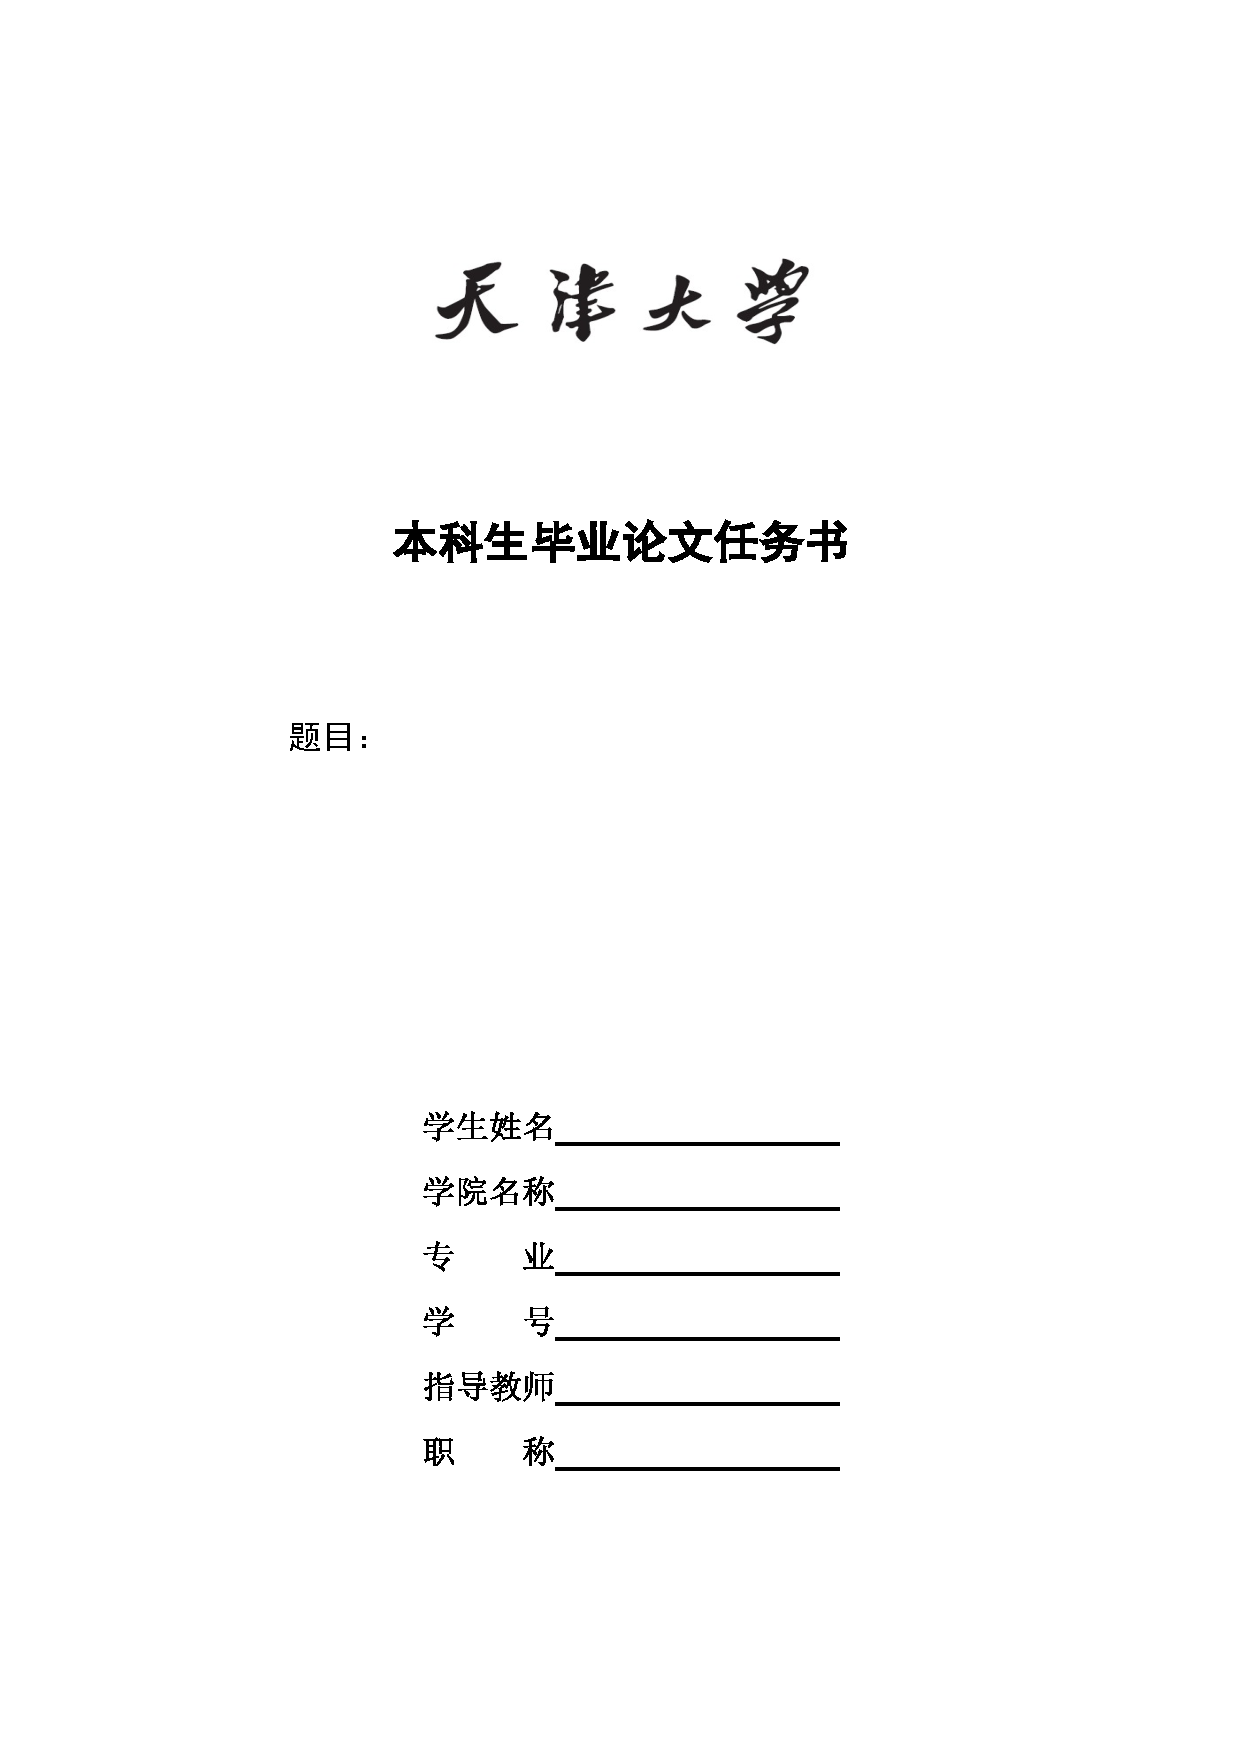
\includepdf[pages=-]{include/task.pdf}

%%%%%%%%%%  开题报告  %%%%%%%%%%
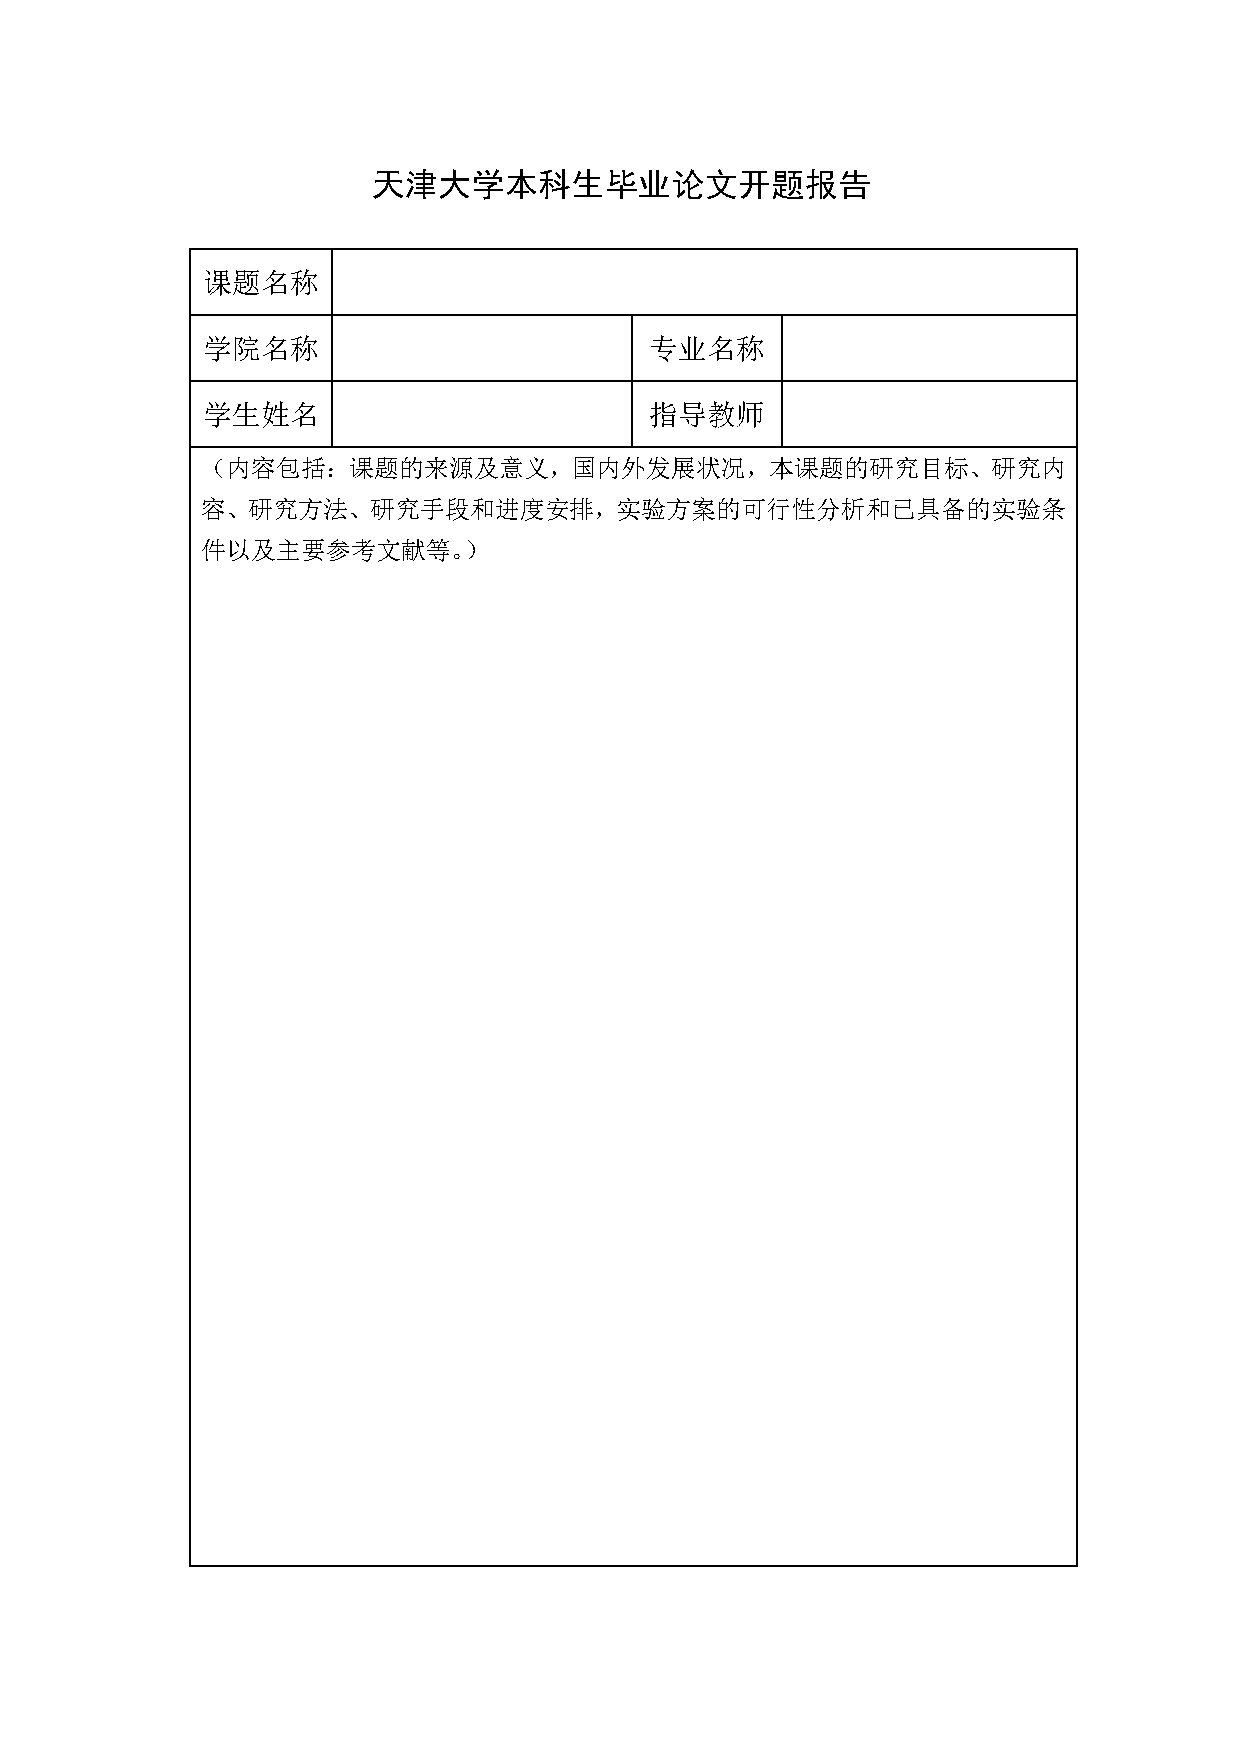
\includepdf[pages=-]{include/open.pdf}

%%%%%%%%%%    摘要    %%%%%%%%%%
% Abstract
\clearpage
\thispagestyle{plain}
\phantomsection
\addcontentsline{toc}{chapter}{Abstract}

\centerline{\zihao{3}\bfseries Abstract}

\linespread{1.4}\zihao{-4}
\bigskip

This thesis explores the relationship between focus structure and pronoun resolution among non-native speakers of English and French. Firstly we reviewed the existing literature on the mechanism of focus effect and pronoun resolution. Then through a self-paced reading test, we find that focus, in the form of cleft structure does not necessarily increase the salience of a informational unit, thus may not in some cases make it a preferred antecedent for pronoun resolution. This result is line with previous researches on this topic. In our experiment, We also find that focused subject in French and focused object in English are processed faster, but focused subjects in both languages leads to longer response time of anaphora. Furthermore, our research also shows that the congruence between anaphora and focus does not make the latter more accessible. In this regard, we argue that the problem of whether there is subject or object preference in English and French is more complicated than the results of current studies.

\bigskip
\noindent\textbf{\zihao{4} Keywords:} 
focus effect, pronoun resolution, self-paced reading, English, French



\setcounter{page}{1}							% 单独从 1 开始编页码
%\pagenumbering{arabic}
%%%%%%%%%%    目录    %%%%%%%%%%
\makecontents

\setcounter{page}{1}							% 单独从 1 开始编页码
%%%%%%%%%%    正文    %%%%%%%%%%
\titleformat{\chapter}{\centering\xiaosan\hei}{\chaptername}{2em}{} % "第~章"小三号黑体居中
% !Mode:: "TeX:UTF-8"

\chapter{绪论}
《他改变了中国:江泽民传》(如图~\ref{book}~所示)这本传记介绍了江泽民同志的人生历程,尤其是阐述和评价了江泽民同志担任中国主要领导人的10多年中创立的历史功绩。在着重于国事活动的同时,也广泛涉及家庭生活、业余爱好、人品风格等方方面面,多角度、多侧面地展现了传主的风采。

	\begin{figure}[htbp!]
		\centering
		
\includegraphics[width=0.5\textwidth]{figures/The_Man_Who_Changed_China.png}
		\caption{红宝书封面}\label{book}
		\vspace{-1em}
	\end{figure}	



\chapter{怒斥记者}
我觉得你们啊,你们……我感觉你们新闻界还要学习一个,你们非常熟悉西方的这一套value。你们毕竟还图样,明白这意思吧。我告诉你们我是身经百战了,见得多啦!啊,西方的哪一个国家我没去过?媒体他们——你……你们要知道,美国的华莱士,那比你们不知道高到哪里去了。啊,我跟他谈笑风生!所以说媒体啊,要……还是要提高自己的姿势水平!懂我的意思——识得唔识得啊?唉,我也给你们着急啊,真的。你们真的……我以为……遍地……你们有一个好,全世界跑到什么地方,你们比其他的西方记者啊,跑得还快。但是呢,问来问去的问题啊,都图森破,啊,上台拿衣服!懂了没有啊?识得唔识得啊?

我很抱歉,我今天是作为一个长者给你们讲的。我不是新闻工作者,但是我见得太多了,我……我有这个必要告诉你们一点,人生的经验。我刚才呢……我刚才我很想啊,就是我每一次碰到你们我就讲中国有一句话叫“闷声大发财”,我就什么话也不说。这是坠吼滴!但是我想,我见到你们这样热情啊,一句话不说也不好。所以你刚才你一定要——在宣传上将来如果你们报道上有偏差,你们要负责的。我没有说要钦定,没有任何这个意思。但是你问……你一定要非得要问我……对董先生姿瓷不姿瓷。我们不姿瓷他?他现在是当特首,我们怎么能不姿瓷特首?对不对?

\begin{table}[htbp]
	\caption{长者用语对照表}\label{table}
	\vspace{0.5em}\centering\wuhao
	\begin{tabular}{ccccc}
		\toprule[1.5pt]
		原文 & 翻译 \\
		\midrule[1pt]
		吼哇 & 好啊 \\
		姿瓷 & 支持 \\
		姿势水平 & 知识水平 \\
		图样 & too young \\
		图森破 & too simple \\
		上台拿衣服 & sometimes naive \\
		识得唔识得啊 & 知道不知道啊 \\
		捉鸡 & 着急 \\
		这是坠吼滴 & 这是最好的 \\
		安格瑞 & angry \\
		一颗赛艇 & excited \\
		\bottomrule[1.5pt]
	\end{tabular}
	\vspace{\baselineskip}
\end{table}



\chapter{视察二院}
\section{我的经历}
我的这个经历就是到了上海,到了89年的年初的时候,我在想我估计是快要离休了,我想我应该去当教授。于是我就给朱物华校长、张钟俊院长,给他们写了一个报告。他们说欢迎你来,不过,这个Apply for Professor,你要去做一个报告。我就做了一个能源与发展趋势的主要的节能措施\citeup{江泽民1989能源发展趋势及主要节能措施},这个报告经过好几百个教授一致通过。那么上海交大教授当了以后我就做第二个报告,就是微电子工业的发展\citeup{江泽民1989论世界电子信息产业发展的新特点与我国的发展战略问题}。这两个报告做了以后不久,过后,1989年的5月31号北京就把我调到北京去了。现在这个报告做了快20年了,所以呢我就去年呢在我们交大的学报,我发表了两篇文章\citeup{江泽民2008对中国能源问题的思考,江泽民2008新时期我国信息技术产业的发展},就是呼应这个89年的报告的。特别是昨天晚上,他又把我这个第二篇报告,还有我这十几年包括在电子工业部、上海市所做的有关于信息产业化的文章,总共我听他们讲是27篇……我也没有什么别的东西送给你们,我们拿来以后我叫钱秘书啊,就把这两个学报,两个学报的英文本——因为他们这里洋文好的人多得很哪——英文本,还有前面出过两本书,再加上昨天晚上出的这本书,送给郭伟华同志,给你送过来,那么给你们作为一个纪念。

\section{不可预料}
人呐就都不知道,自己就不可以预料。一个人的命运啊,当然要靠自我奋斗,但是也要考虑到历史的行程。我绝对不知道,我作为一个上海市委书记怎么把我选到北京去了,所以邓小平同志跟我讲话,说“中央都决定啦,你来当总书记”,我说另请高明吧。我实在我也不是谦虚,我一个上海市委书记怎么到北京来了呢?但是呢,小平同志讲“大家已经研究决定了”,所以后来我就念了两首诗,叫“苟利国家生死以,岂因祸福避趋之”,那么所以我就到了北京。

\section{三件小事}
到了北京我干了这十几年也没有什么别的,大概三件事:

\begin{itemize}
	\item 一个,确立了社会主义市场经济;
	\item 第二个,把邓小平的理论列入了党章;
	\item 第三个,就是我们知道的“三个代表”。
\end{itemize}

如果说还有一点什么成绩就是军队一律不得经商!这个对军队的命运有很大的关系。因为我后来又干了一年零八个月,等于我在部队干了15年军委主席。还有九八年的抗洪也是很大的。但这些都是次要的,我主要的我就是三件事情,很惭愧,就做了一点微小的工作,谢谢大家。



\chapter{谈笑风生}
新闻、媒体也是企业,它们不是非赢利组织,而是以赢利为目的的商业企业。新闻是这些企业制造的产品,它们想用新闻这个产品去赚钱,它们就有充分的动机弄虚做假、以次充好、串谋合谋、唯利是图。凭什么新闻这个产品的质量就可以不受监管、不受控制呢?在新闻质量和新闻消费者之间不是一样存在一个信息非对称问题吗?看来,美国这个先进国家还没有想出监管新闻这种产品的好办法来,就象你们在30年代以前对商业自由那样,既然如此,我们有什么必要匆匆忙忙去抄袭你们呢?还是等你创造出更好的经验后,我们再去学习吧。

至于个人自由,任何人的绝对自由都是对别人的限制。美国南部有个工厂,白种工人在车上画着南方联邦的旗帜,非裔工人向厂方提出抗议,厂方同意不让这些车进厂门,白种工人又抗议他们的言论自由受到侵害。倒底谁应该有言论自由的权力呢?双方都有就会产生冲突,一方有,另一方就会受到限制。有一个人烧了美国国旗,地方法院要起诉他,最高法院认为这个人无罪,因为他有言论自由的权力。而美国国会的一些议员不干了,他们要立法使这个人有罪。倒底谁说的对呢?所谓言论自由,本质上是一个博奕论难题,没有正确的解,所以要用民主集中制来限制它。

民主就是多数原则,是用多数人的自由限制少数人的自由。集中是由多数人的代表来行使多数权力,本质上是多数人中的少数人限制多数人的自由。之所以个人自由必须受到限制,是因为还存在一个效率原则。所以在一个社会中,效率和公正不可偏废,当效率和公正相抵触时,必须实行效率优先原则,这就是历史的逻辑,或者称为历史悖论。看来华莱士先生不太懂历史和哲学,我就请教一个数学问题,已知
\begin{align}
	f(a,b,c)=abc(100a+10b+c)\label{func}
\end{align}

其中\(a,b,c\in \mathbb{N}^+\)且\(a>b>c\),求函数~\eqref{func}~的值域。

	


\chapter{结论}
我们党要始终代表中国先进生产力的发展要求——就是党的理论、路线、纲领、方针、政策和各项工作,必须努力符合生产力发展的规律,体现不断推动社会生产力的解放和发展的要求,尤其要体现推动先进生产力发展的要求,通过发展生产力不断提高人民群众的生活水平;

我们党要始终代表中国先进文化的前进方向——就是党的理论、路线、纲领、方针、政策和各项工作,必须努力体现发展面向现代化、面向世界、面向未来的,民族的科学的大众的社会主义文化的要求,促进全民族思想道德素质和科学文化素质的不断提高,为我国经济发展和社会进步提供精神动力和智力支持;

我们党要始终代表中国最广大人民的根本利益——就是党的理论、路线、纲领、方针、政策和各项工作,必须坚持把人民的根本利益作为出发点和归宿,充分发挥人民群众的积极性主动性创造性,在社会不断发展进步的基础上,使人民群众不断获得切实的经济、政治、文化利益。

%%%%%%%%%%  参考文献  %%%%%%%%%%
\makereferences

%%%%%%%%%%    附录    %%%%%%%%%%
\titleformat{\chapter}{\centering\sihao\hei}{\chaptername}{2em}{} % 标题四号黑体居中
% !Mode:: "TeX:UTF-8"

\titlecontents{chapter}[2em]{\vspace{.5\baselineskip}\xiaosan\song}%
             {\prechaptername\CJKnumber{\thecontentslabel}\postchaptername\qquad}{} %
             {}             % 设置该选项为空是为了不让目录中显示页码          
\addcontentsline{toc}{chapter}{外文资料}
%\setcounter{page}{1}       % 如果需要从该页开始从 1 开始编页,则取消该注释
\markboth{外文资料}{外文资料}
\chapter*{外文资料}

\trtitle{Gettysburg Address}

Four score and seven years ago our fathers brought forth on this continent, a new nation, conceived in Liberty, and dedicated to the proposition that all men are created equal.

Now we are engaged in a great civil war, testing whether that nation, or any nation so conceived and so dedicated, can long endure. We are met on a great battle-field of that war. We have come to dedicate a portion of that field, as a final resting place for those who here gave their lives that that nation might live. It is altogether fitting and proper that we should do this.

But, in a larger sense, we can not dedicate—we can not consecrate—we can not hallow—this ground. The brave men, living and dead, who struggled here, have consecrated it, far above our poor power to add or detract. The world will little note, nor long remember what we say here, but it can never forget what they did here. It is for us the living, rather, to be dedicated here to the unfinished work which they who fought here have thus far so nobly advanced. It is rather for us to be here dedicated to the great task remaining before us—that from these honored dead we take increased devotion to that cause for which they gave the last full measure of devotion—that we here highly resolve that these dead shall not have died in vain—that this nation, under God, shall have a new birth of freedom—and that government of the people, by the people, for the people, shall not perish from the earth.				% 外文资料
% !Mode:: "TeX:UTF-8"

\titlecontents{chapter}[2em]{\vspace{.5\baselineskip}\xiaosan\song}
             {\prechaptername\CJKnumber{\thecontentslabel}\postchaptername\qquad}{}
             {}             % 设置该选项为空是为了不让目录中显示页码
\addcontentsline{toc}{chapter}{中文译文}
\setcounter{page}{1}            % 单独从 1 开始编页码
\markboth{中文译文}{中文译文}   % 用于将章节号添加到页眉中
\chapter*{中文译文}

\trtitle{葛底斯堡演说}

87年前,我们的先辈们在这个大陆上接生了一个新型的共和国,她受孕于自由的理念,并献身于一切人生来平等的理想。

现在我们进行了一场重大的内战,以考验这个共和国,或者任何一个受孕于自由和献身于上述理想的共和国是否能够长久生存下去。我们站在这场战争中的一个重要战场上聚集。烈士们为使这个共和国能够生存下去而献出了自己的生命,我们来到这里,是要把这个战场的一部分奉献给他们作为最后安息之所。我们这样做是完全应该而且是非常恰当的。但是,从更广泛的意义上来说,这块土地我们不能够奉献,不能够圣化,不能够神化。正是那些活着的或者已经死去的曾经在这里战斗过的英雄们才使得这块土地成为神圣之土。我们无力使之增减一分。我们在这里说什么,世人不会注意,也不会长期记住,但是英雄们的行为永远不会被人们遗忘。

这更要求我们这些活着的人去继续英雄们为之战斗,并使之前进的未尽事业。倒是我们应该在这里把自己奉献于仍然留在我们面前的伟大任务——我们要从这些光荣的死者身上汲取更多的献身精神,来完成他们已经完全彻底为之献身的事业;我们要在这里下定最大的决心,不让这些死者白白牺牲;我们要使共和国在上帝保佑下得到自由的新生,要使这个民有、民治、民享的政府永世长存。				% 中文译文
\defaultfont

\BiAppendixChapter{��~~~~л}{Acknowledgement}

\ifxueweidoctor               %��ʿҳü
\fancyhead[CO]{\CJKfamily{song}\xiaowu\leftmark}
\else
\fancyhead[CO]{\CJKfamily{song}\xiaowu ��������ҵ��ѧ\cxueke \cxuewei ѧλ����}
\fi
\fancyhead[CE]{\CJKfamily{song}\xiaowu ��������ҵ��ѧ\cxueke \cxuewei ѧλ���� }%

������ģ����UFO@bbs.hit.edu.cn�ġ���������ҵ��ѧ��ѧ��ʿ��˶ʿ������ģ�塷�Ļ����ϣ�
���ںܶ��˵İ�������ɵģ��ڴ�һ�������DZ�ʾ��л��

�ر��лStanley����������ģ�忪Դ��ĿPluto�Լ���������ģ��Ĵ����޸ģ�
ʹ֮���ӷ��Ϲ�������ģ��Ҫ��

�ر��л�������϶���վ��~Tex~�İ���~Tex��nebula������cucme��
������ʼ���ն�ȫ��֧��ģ�����������Ϊ�����˴����Ĺ�����

��л���괺~(HIT bbs ID: dengnch)�������˴�����ʱ��������ģ���
һϵ�в�����ʹ�ø�~\LaTeX~ģ��Ͷ�Ӧ��~Word~ģ��ĸ�ʽ������ȫһ�¡�

��лˮľ�廪��~\TeX~��~\LaTeX~��ĸ�λ����Ϊ���ṩ�ĸ��ְ�����
�ر���~snoopyzhao~���ѣ���������ĵ�Ϊ��ģ�����������ѣ�ʹ��ģ�����������
˳�����С�

������ĸ�л�������϶���~bbs~վ~Tex~���������ѵĴ���֧�֣�



ֵ���������֮�ʣ������������˽��������ʦ��ͬѧ�����Գ�ֿ��л�⣡

���ȸ�л�ҵĵ�ʦ{\bf ijijij}���ڣ������ĵ��о�����������{\bf
ij}��ʦ����Ľ�����չ���ġ�
����ѧ���ϲ��Ͻ�ȡ������������ִ��׷��ľ�������ѧϰ�İ�����{\bf
ij}��ʦ��������̵���ʶ������dz���Ľ�������������ӡ��


��л{\bf ijijij}���ں�{\bf ijijij}���ڶ���ѧϰ�͹����İ�����
�����ڷܵĹ������硢��۵�����̬�ȶ�����ظ�Ⱦ���ҡ���л{\bf
ijijij}���ں�{\bf ijijij}���ڶ���ѧҵ�������ϵĹ��ġ�


��л��ʿ��{\bf ijijij}��{\bf ijijij}��{\bf ijijij}��{\bf ijijij}��
���ҵ���˽�����ͻ���֧�֡���лʵ�������е��ֵܽ����ǣ�
����Ҷȹ����ⳤ�õ�ѧϰ���о��׶Σ������ҽ�����⣬����˼�롣

����ر�Ҫ��л�ҵ������ǣ����Ƕ���Ҫ�����٣��������ҵĶ��ǹػ���֧�ֺ����⡣
				% 致谢
\clearpage
\end{document}									% 结束全文
